\documentclass[]{article}
\usepackage{metalogo} % for the logo of XeLaTeX
\usepackage{xeCJK}
\usepackage{enumerate}
\usepackage{booktabs}
\usepackage{amsmath}
\usepackage{indentfirst}
\usepackage{cite}
\usepackage{algorithm}
\usepackage{algorithmicx}
\usepackage{algpseudocode}
%opening
\title{一套农家乐信息管理系统的设计}
\author{尹达恒}

\begin{document}
	\pagenumbering{Roman}
	\maketitle
	\newpage
	\begin{abstract}
		为提高农家乐信息管理效率,帮助游客更有效地选择合适的农家乐游玩,开发了该管理系统。通过需求分析、系统逻辑结构设计、编码实现等过程,对农家乐信息管理系统从农家乐商户和游客两个角度进行了具体设计,并开发了农家乐游客公开评价的的管理模式。主要功能包括商户信息认证、商户和游客信息管理、分地域农家乐检索、游客评价等。该系统可以在一定程度上缓解国内农家乐市场服务质量良莠不齐、农家乐商户和游客信息不对称的问题能够有效提高政府对农家乐市场的管理效率,帮助游客方便的查询农家乐信息,具有一定的创新性和实用性。
		
		\textbf{关键字:}待定
	\end{abstract}
	\newpage
	\tableofcontents
	\newpage
	\pagenumbering{arabic}
	\section{引言}
	改革开发以来,国内物质生产水平和居民收入不断提高,人民的物质生活越来越富足;但与此同时,在中国的各大城市,对工作效率和业绩的追求也使人们的生活节奏全面“提速”。越是生活在大城市的人们,越是发现在工作之余可支配的时间越来越少\cite{RN38}。工作压力大长时间地在封闭的室内工作、缺乏运动、熬夜、生活不规律等诸多快节奏生活中的不良习惯使许多人出现身体亚健康或者“三高” 问题, 如何更好地预防或者改善这些症状是很多人面临的问题,在这样的背景下,一股“逃离城市,返璞归真”的热潮正悄然兴起,社会对“休闲+养生”农业的需求不断增\cite{RN5}\cite{RN39}。农家乐作为暂时远离城市繁杂纷扰,追求“休闲+养生”的乡村宁静生活的理想去处,自然也越来越受城市居民的青睐。与此同时,在城市附近飞速扩张的农家乐市场也极大地促进了乡村经济的发展。其积极影响主要包括促进乡村就业、拓宽乡村收入来源、提升乡村劳动人口素质、优化乡村基本设施建设等诸多方面\cite{RN17}。然而,农家乐市场的快速扩张也使得当前各地农家乐种类繁多,服务质量良莠不齐。游客在选择农家乐时有较大的盲目性,不知道各个农家乐实际的服务质量如何,也不知道哪个农家乐适合自己,很容易被某些农家乐广告上与实际情况不符的图片和描述所欺骗,不仅达不到放松的目的,反而会因为农家乐服务质量不佳而影响心情,徒增烦恼。当前农家乐市场存在着许多问题:市场上农家乐的旅游产品大都大同小异,缺乏特色,一些农家乐甚至都不再采用自家种植、养殖的 蔬菜和肉类,而是直接在附近集市上购买;基础设施建设仍然难以跟上发展脚步;经营理念落后;经营安全意识较低,卫生意识淡薄\cite{RN28}\cite{RN23}。更重要的是,由于农家乐大都采用独立产权运营模式,对于农家乐的服务质量很难建立一个统一的评价指标,许多农家乐为了招揽客户,在广告上放上大量夸张甚至与实际情况不符的图片和描述,或是利用农家乐地处较为偏远的条件,用较低的入门价格诱使顾客前往,而后故意抬高餐饮和一些生活必须品的价格,影响用户体验。为了规范农家乐市场的健康发展,建立一套具有评价和筛选功能的农家乐信息管理系统势在必行。本文提出的一套农家乐信息管理系统采用基于用户感知的质量评价体系\cite{RN40},实现了面向商户和游客的两种客户端,商户端方便农家乐商户对自己的服务和产品进行宣传,也方便政府部门对农家乐的广告宣传进行审核和管理;游客端可以对查看农家乐商户的确切服务和评级信息、按照区域和评级对农家乐商户进行检索,查看其他用户对商户的评价,并在实际体验后对农家乐进行评价。通过农家乐商户在注册时输入到系统中的信息,市场管理人员可以很方便地知道农家乐商户的具体情况,并通过游客对农家乐商户的评价信息进行比对及时发现农家乐商户在经营过程中的不良行为从而进行精确整治;旅客也可以通过农家乐商户的信息和其他旅客的评价选择适合自己的农家乐商户,从而更好地体验“休闲+养生”的乡村宁静生活,更有效地提高生活舒适度和满意度。
	\section{系统设计}
	\subsection{需求分析}
	\subsubsection{用户需求分析}
	\begin{enumerate}
		\item 政府部门需求分析:
		
		很多地区的农家乐市场还处在起步阶段,政府部门尚未对农家乐市场有一个全面统一的规划,尚未建立一个有效的渠道准确而及时地了解农家乐商户的具体情况,进而也就缺乏对农家乐创业的政策、资金和基础设施建设的支持,这些都限制了农家乐旅游的发展\cite{RN31}。建立一个统一的与农家乐对接的信息集中、市场管理和经营引导平台,对农家乐市场分布的经营情况有一个整体的把握,进行全面的布局和规划是当前亟待解决的难题。
		除经济部门对农家乐商户创业进行经营支持外,市场监管部门也需要对农家乐市场中的各商户的服务质量进行监督。但当前市场监管部门同时也缺乏一个能与游客对接的农家乐质量评价平台,难以基于实际用户体验对农家乐的服务质量进行客观的评估。许多地方的农家乐出现了服务质量下降、虚假宣传、恶意抬高商品价格等不良行为,放任这些不良行为势必会对市场信誉和地区经济造成严重损害。建立一个信息平台以使监管部门能从游客处获取对农家乐实际服务情况的评价并对农家乐服务质量进行客观评估迫在眉睫。
		
		\item 农家乐商户需求分析:
		
		在很多地方,农家乐的经营模式仍在摸索之中,从业者之间信息流动缓慢,农家乐创业和经营的经验一些重要的市场变化信息难以在从业者之间有效地传播,导致一些地区农家乐项目同质化严重,重复开发的农家乐项目充斥市场,农家乐创业成功率得不到有效提高\cite{RN31}。为使得农家乐商户、创业者以及优秀的农家乐创业和投资项目快速与政府、相关企业和投资者实现对接,得到投资和发展机会,一个统一的农家乐商户信息交流平台必不可少。
		
		\item 游客需求分析:
		
		如今,市场上的农家乐服务种类繁多,对农家乐旅游不同的游客都有自己的需求。在一个统一的信息平台进行农家乐信息检索,方便快捷地获取所需的农家乐信息继而选择喜欢的农家乐进行消费将极大的优化游客的旅游消费体验。
	\end{enumerate}
	\subsubsection{功能需求分析}
	农家乐信息管理系统是根据农家乐市场管理和游客查询的需要而建立的数据库系统。网页界面为农家乐商户和游客提供方便简洁的可视化操作,用户(农家乐商户或游客)通过账号密码登录验证,依据不同角色进入不同的界面。
	
	对于农家乐商户,可以进行如下操作:
	\begin{enumerate}
		\item 注册商户信息:用户通过录入必要信息并上传有效经验证件进行注册,注册后的商户可在系统中被游客检索到。
		\item 编辑商户描述:注册后的商户可以在商户主页修改商铺描述文字,上传和删除商铺描述图片。
		\item 查看用户评价:注册后的商户可以在商户主界面看到已消费的游客对店铺发表的评价。
		\item 检索其他商户信息:注册后的商户可以在检索页面检索并查看其他商户的店铺注册信息、商户描述和用户评论。
	\end{enumerate}
	
	对于农家乐游客,可以进行如下操作:
	\begin{enumerate}
		\item 注册个人信息:用户录入必要的个人信息进行注册。
		\item 检索其他商户信息:注册后的用户可以在检索页面检索并查看商户的店铺注册信息、商户描述和用户评论。
		\item 发表评价:已注册的用户在农家乐消费完成后可以在对应店铺的主界面下发表公开评价。
	\end{enumerate}
	
	对于系统管理员,可以进行如下操作:
	\begin{enumerate}
		\item 操作店铺信息:管理员可以增删改查数据库中的店铺信息,,删除或修改不合规范的店铺。
		\item 操作用户信息:管理员可以增删改查数据库中的用户信息,封禁不良用户。
		\item 操作评价信息:管理员可以增删改查数据库中的用户评价,控制恶意评论。
	\end{enumerate}
	
	\subsection{结构设计}
	\subsubsection{逻辑结构设计}
	逻辑设计是把现实世界中的实际需求转化为计算机内的逻辑结构的过程,是数据库和网站业务逻辑设计的重要组成部分。基于E-R模型的数据库逻辑结构设计方法因不受实际数据库结构的制约,且结构清晰直观而广受欢迎\cite{RN41}。本系统的数据库逻辑结构也使用基于E-R模型的方法进行设计。根据需求分析的结果,可以抽象出用户、商户、评价三类实体,各实体之间的E-R模式见图\ref{ER}。
	\begin{figure}
		\centering
		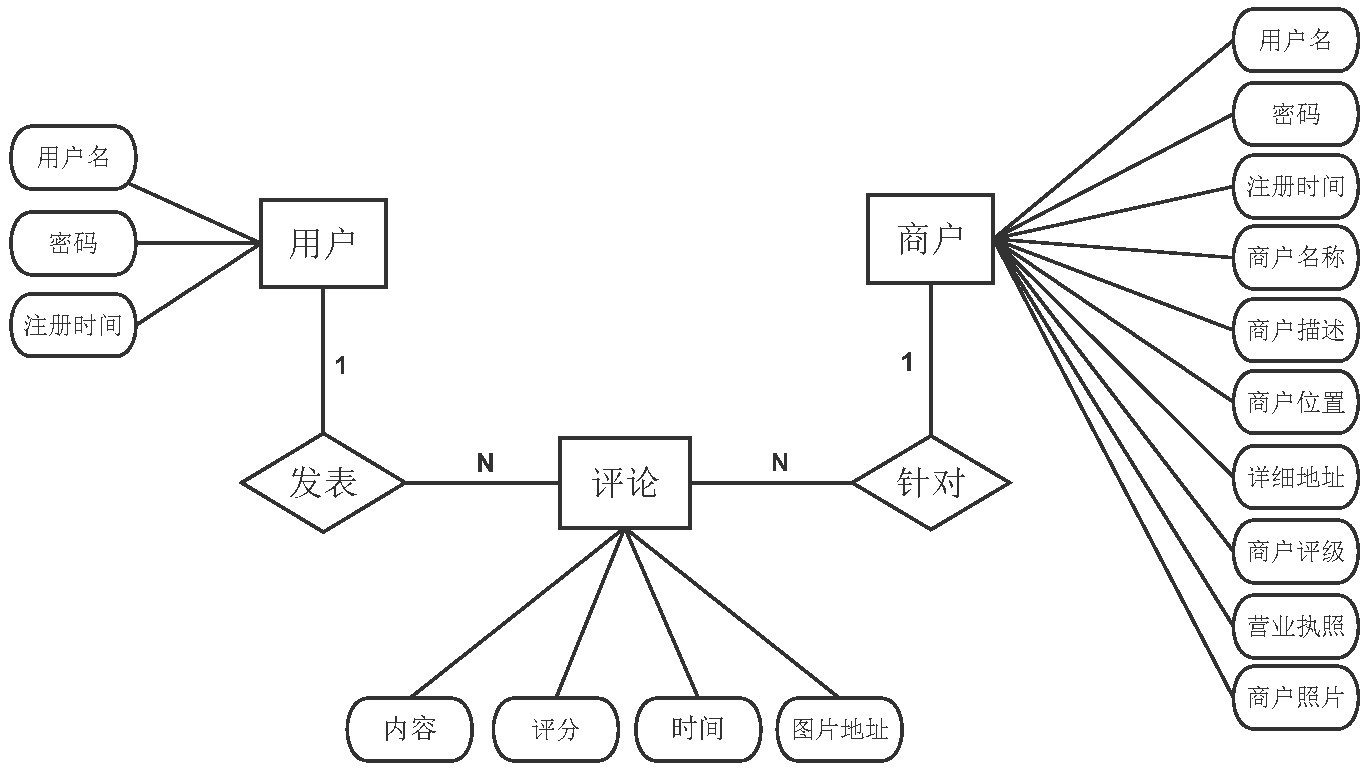
\includegraphics[width=\textwidth, keepaspectratio]{figures/ER.pdf}\\
		\caption{农家乐信息管理系统E-R图}
		\label{ER}
	\end{figure}
	\subsubsection{数据结构设计}
	数据结构设计是逻辑结构向计算机内的数据存储方式转化的过程,也是软件系统设计从逻辑层面落实到数据层面的过程。一个有效的、规范化的数据结构不但可以简化系统的设计和维护过程,更能在实际应用中加快系统的运行速度\cite{RN42}。数据库系统中数据结构的设计一般遵循三个范式(NF):\cite{RN43}
	
	\begin{enumerate}
		\item 1NF:数据表每一列都是不可分割的基本数据项。
		\item 2NF:满足1NF且数据表的每一行都能被一个主关键字(primary key)唯一区分。
		\item 3NF:每个数据表的非主关键字都不包含其它表中已包含的信息。
	\end{enumerate}
	
	一个结构良好的、低冗余度的、不容易出现插入异常和更新异常的关系型数据库应尽可能地遵循关系数据库设计的三个范式\cite{RN44}。
	
	在本系统的设计中,数据结构设计要做的就是按照关系数据库的三个范式把表现逻辑结构的E-R模型转化为数据库中的表结构,并对其进行优化,从而能进一步转化为数据库结构化查询语言(SQL)用于系统实现时构建数据库。本系统中的E-R模型关系实体转化而成数据结构包括三个表结构以及两个外键。其中表结构组成及功能如下:
	
	\begin{enumerate}
		\item 用户信息表(表\ref{用户}):存储用户的用户名、密码、注册时间。
		\item 商户信息表(表\ref{商户}):存储商户的用户名(登录名)、密码、注册时间、以及商铺的信息(商户名称、商户描述、商户位置、详细地址、商户评级、营业执照、商户照片)。
		\item 评价信息表(表\ref{评价}):存储用户对商户评价信息,包括给出评价的用户、接受评价的商户、评价内容、评价中给出的分数、评价时间和评价图片。
	\end{enumerate}
	
	两个外键约束(表\ref{外键})确保评价信息表中给出的给出评价的用户和接受评价的商户在系统中确实存在。

	\begin{table}[!hbp]
		\centering
		\caption{用户信息表}\label{用户}
		\begin{tabular}{|c|c|c|c|}
			\hline
			数据名称&数据类型&长度&约束条件\\
			\hline
			用户名&varchar&255&not null,primary key\\
			密码&varchar&255&not null\\
			注册时间&datetime&8&not null\\
			\hline
		\end{tabular}
	\end{table}
	\begin{table}[!hbp]
		\centering
		\caption{商户信息表}\label{商户}
		\begin{tabular}{|c|c|c|c|}
			\hline
			数据名称&数据类型&长度&约束条件\\
			\hline
			用户名&varchar&255&not null,primary key\\
			密码&varchar&255&not null\\
			注册时间&datetime&8&not null\\
			商户名称&varchar&255&not null\\
			商户描述&varchar&255&not null\\
			商户位置&varchar&255&not null\\
			详细地址&varchar&255&not null\\
			商户评级&tinyint&1&not null\\
			营业执照&varchar&255&not null,文件路径\\
			商户照片&varchar&255&not null,文件路径\\
			\hline
		\end{tabular}
	\end{table}
	\begin{table}[!hbp]
		\centering
		\caption{评价信息表}\label{评价}
		\begin{tabular}{|c|c|c|c|}
			\hline
			数据名称&数据类型&长度&约束条件\\
			\hline
			id&bigint&8&not null,primary key,auto\_increment\\
			用户&varchar&255&not null,\\
			商户&varchar&255&not null\\
			内容&varchar&255&not null\\
			打分&tinyint&1&not null\\
			时间&datetime&8&not null\\
			图片&varchar&255&not null,文件路径\\
			\hline
		\end{tabular}
	\end{table}
	\begin{table}[!hbp]
		\centering
		\caption{外键连接表}\label{外键}
		\begin{tabular}{|c|c|c|c|}
			\hline
			表名&键值&引用表名&引用外键值\\
			\hline
			评价&用户&用户&用户名\\
			评价&商户&商户&用户名\\
			\hline
		\end{tabular}
	\end{table}
	
	根据三个范式对本系统的数据结构进行分析后,三个表结构和外键的设计完全符合三个范式的要求,因此是结构良好的、低冗余度的、不容易出现插入异常和更新异常的关系型数据库。
	\section{系统实现}
	本系统以MySQL作为数据库平台,以PHP作为开发语言开发。PHP语言混合了C、Java、Perl的特点并且融合了PHP自创的新语法,且可以比CGI或者Perl更快速的执行动态网页,支持几乎所有流行的数据库以及操作系统,与MySQL数据库结合紧密,是动态网页快速开发的不二选择\cite{RN45}。
	
	本系统基本实现了预期功能,在开发过程中使用的bootstrap框架使系统风格简洁友好;商铺页面(图\ref{page-main})结构清晰、层次分明;PHP和MySQL数据库的结合使查询界面(图\ref{page-search})功能全面而快捷。本系统能够帮助用户便捷有效地获取自己想要的商户信息,具有一定的创新性和实用性。
	
	\begin{figure}
		\centering
		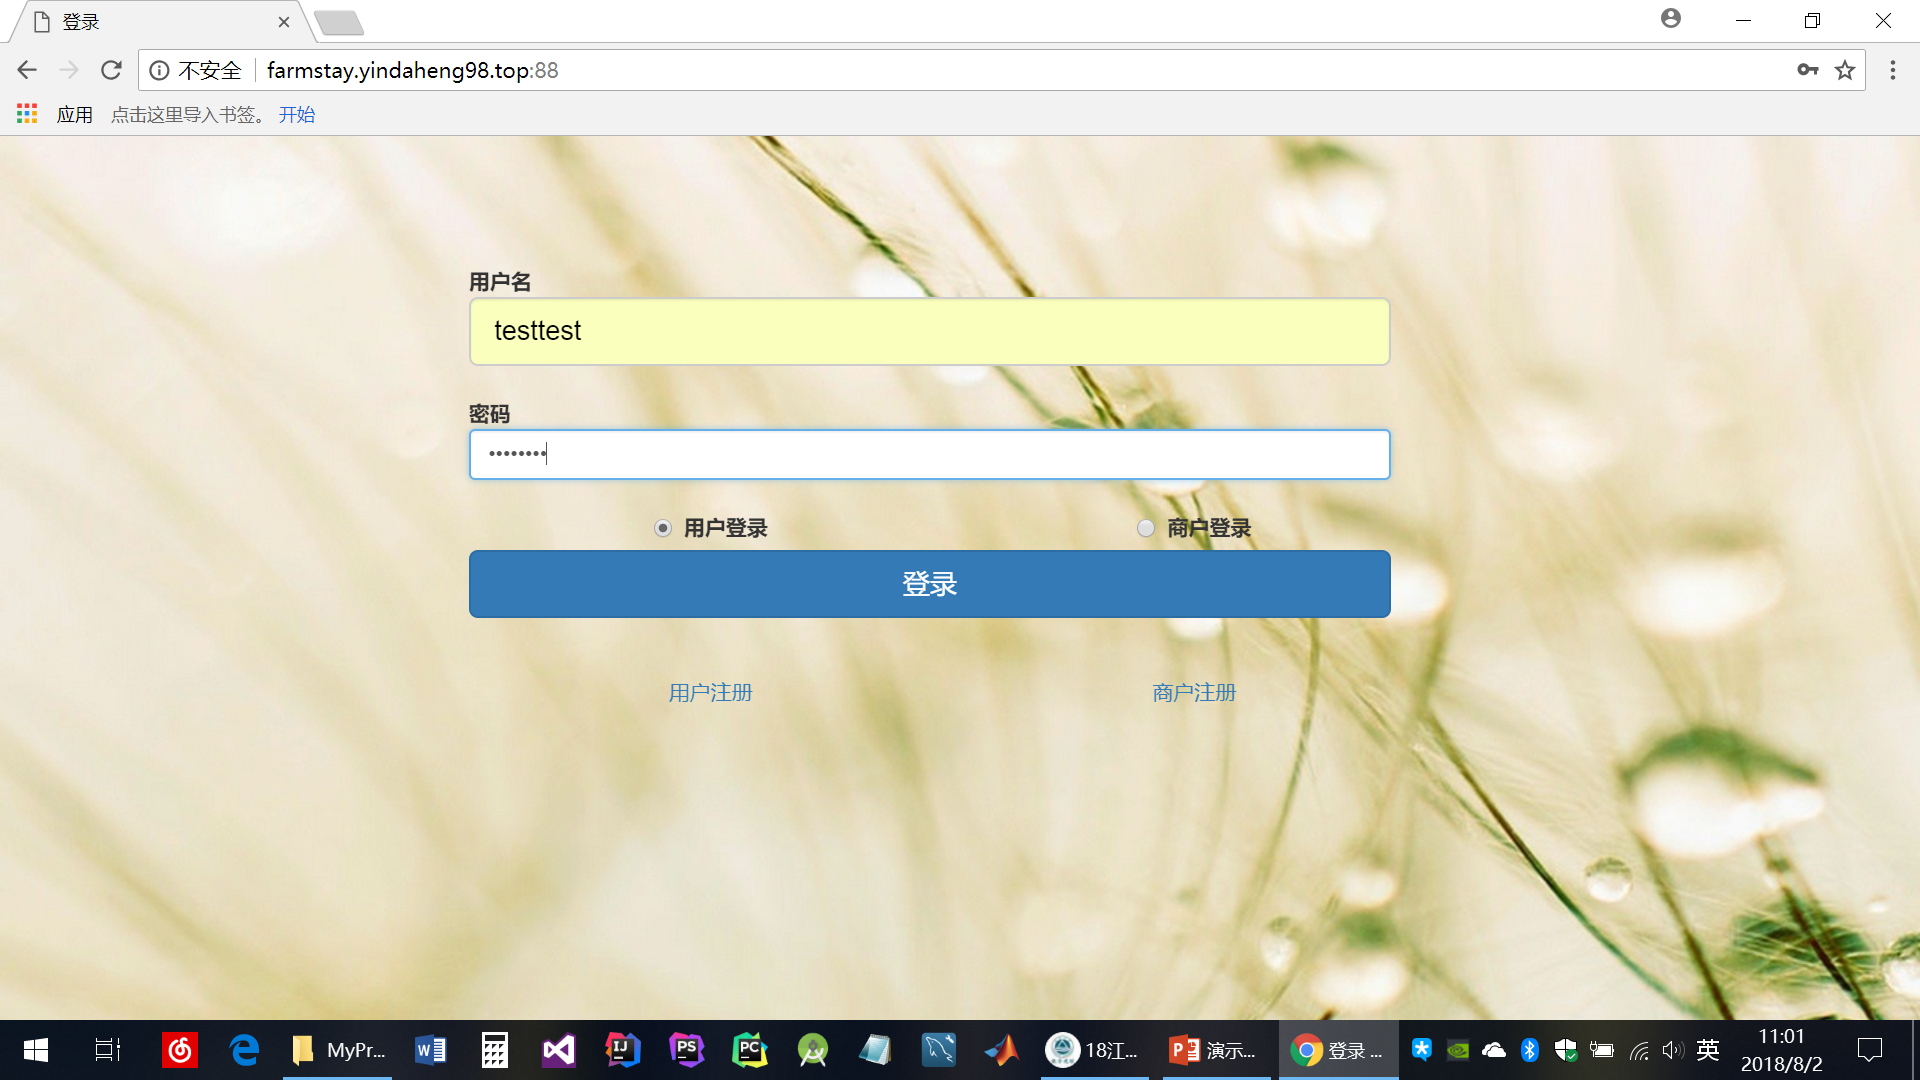
\includegraphics[width=\textwidth, keepaspectratio]{figures/page-main.png}\\
		\caption{商铺页面}\label{page-main}
	\end{figure}
	\begin{figure}
		\centering
		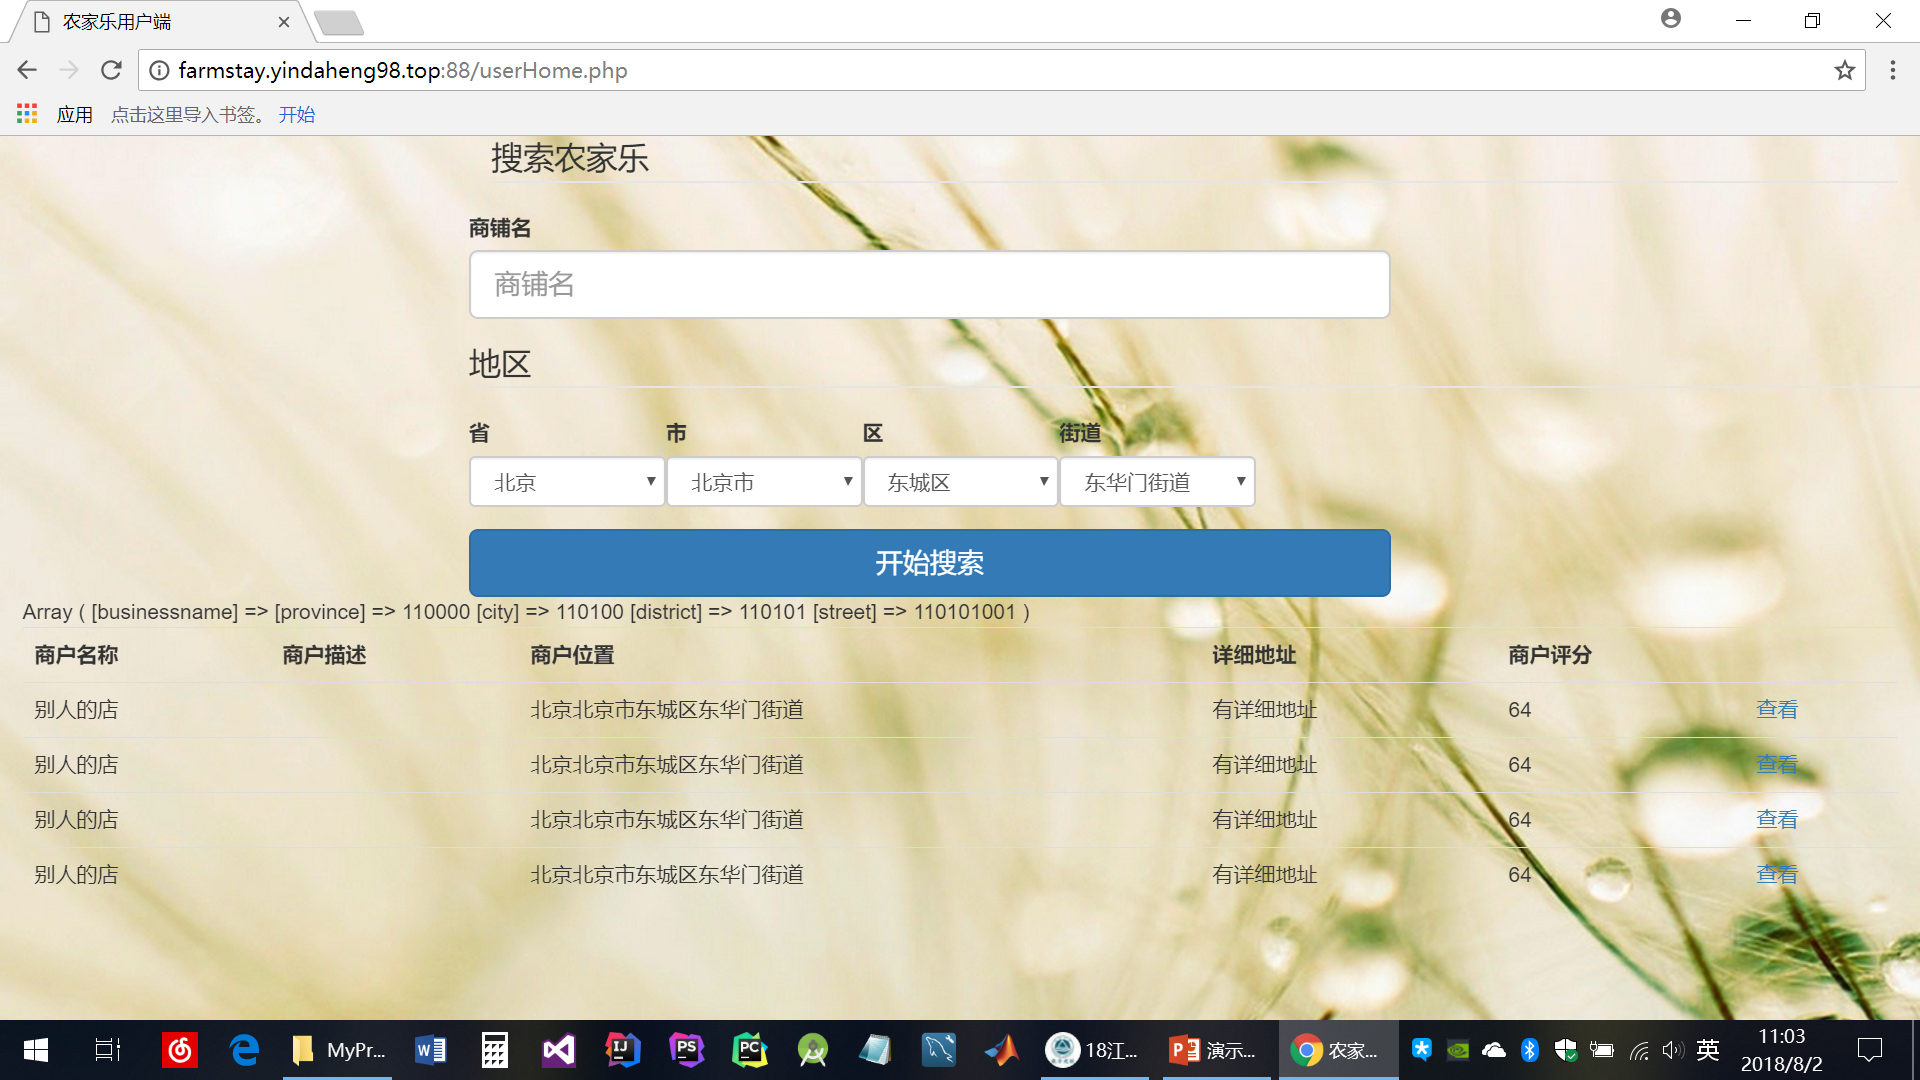
\includegraphics[width=\textwidth, keepaspectratio]{figures/page-search.png}\\
		\caption{查询界面}\label{page-search}
	\end{figure}
	
	\section{优势和应用前景}
	\subsection{优势}
	在本系统中,游客可以根据自己的喜好检索想要的农家乐商户信息,在消费完成后对农家乐商户进行评论和打分,在这个过程中形成的有效数据库信息可以辅助其他游客对良莠不齐的农家乐商户进行筛选,同时也可以帮助市场监管部门及时发现和整治有不良行为的农家乐商户提高农家乐市场监管的针对性和有效性。
	\subsection{应用前景}
	在未来,本系统可以根据需要进行扩展,系统中可以添加更多更方便快捷的检索方式,帮助游客更加快速地检索到自己想要的农家乐商户信息;数据库可以根据农家乐的实际服务内容描述建立同类商户之间的索引,实现关联搜索;系统可以从用户搜索和选择的农家乐商户出发,建立用户消费偏好,主动向用户推送可能感兴趣的相关农家乐商户,促进用户消费。该系统未来可以融合在线上农家乐预约和消费APP中,不仅为用户提供一个方便快捷、富有人性化的农家乐信息查询和消费平台,也为市场监管部门对农家乐市场的监管提供了一条有效途径。
	\section{结语}
	当下农家乐市场监管和信息交流效率低下,大多数农家乐商户还处在单打独斗的阶段,用户也没有一条有效的途径发现优秀的农家乐商户,这造成了农家乐市场的监管空白,阻碍了农家乐市场的规范化和健康发展。本农家乐信息管理系统从农家乐商户和游客的实际需求出发,设计的信息管理模式和评价模式可以缓解监管部门在对农家乐经营情况进行评价时的评价标准问题和游客在选择农家乐商户时的信息缺失问题,同时还能为游客推荐可能感兴趣的农家乐商户,促进消费。此系统对当下农家乐市场的监管和发展起到了一定的帮助和促进作用。
	\bibliographystyle{plain}
	\bibliography{Refs}
\end{document}
